\section{Iterative Auswertung des Kamerabildes}	

	Das Bild der Kamera werden iterativ ausgewertet um die beiden Fahrbahnlinien zu erkennen und daraus ein Ausgangssignal für die Steuerung zu generieren. Der gewählte Ansatz war es, die Fahrbahnlinien durch zwei Geraden anzunähern. Die Funktion HoughLines wird verwendet um die Fahrbahnlinien zu erkennen und die zugehörigen Geraden zu berechnen. Da die Funktion HoughLines in den meisten Fällen nicht nur die beiden Fahrbahnlinien erkennt, sondern alle möglichen Geraden, bestand die erste Aufgabe darin, nur die Geraden herauszufiltern, welche die Fahrbahnlinien repräsentieren, und alle anderen Geraden zu verwerfen. Im Programm wird dies erreicht, indem alle Geraden, die durch die Funktion HoughLines gefunden wurden mit dem Geradenpaar aus dem vorherigen Programmdurchlauf verglichen werden, und nur ähnliche Geraden beibehalten werden.\\
	
	Beim Start des Programm werden für die beiden Geraden feste Werte vorgegeben, die dann korrigiert und an die erkannten Linien angepasst werden. In Abbildung \ref{fig:fahrbahn} ist dies bildlich dargestellt. Die roten Linien sind zu Beginn des Programms fest vorgegeben. Die blauen Linien sind das Ergebnis der Korrektur durch das Programm.
	
	\begin{figure}[H]
		\centering
		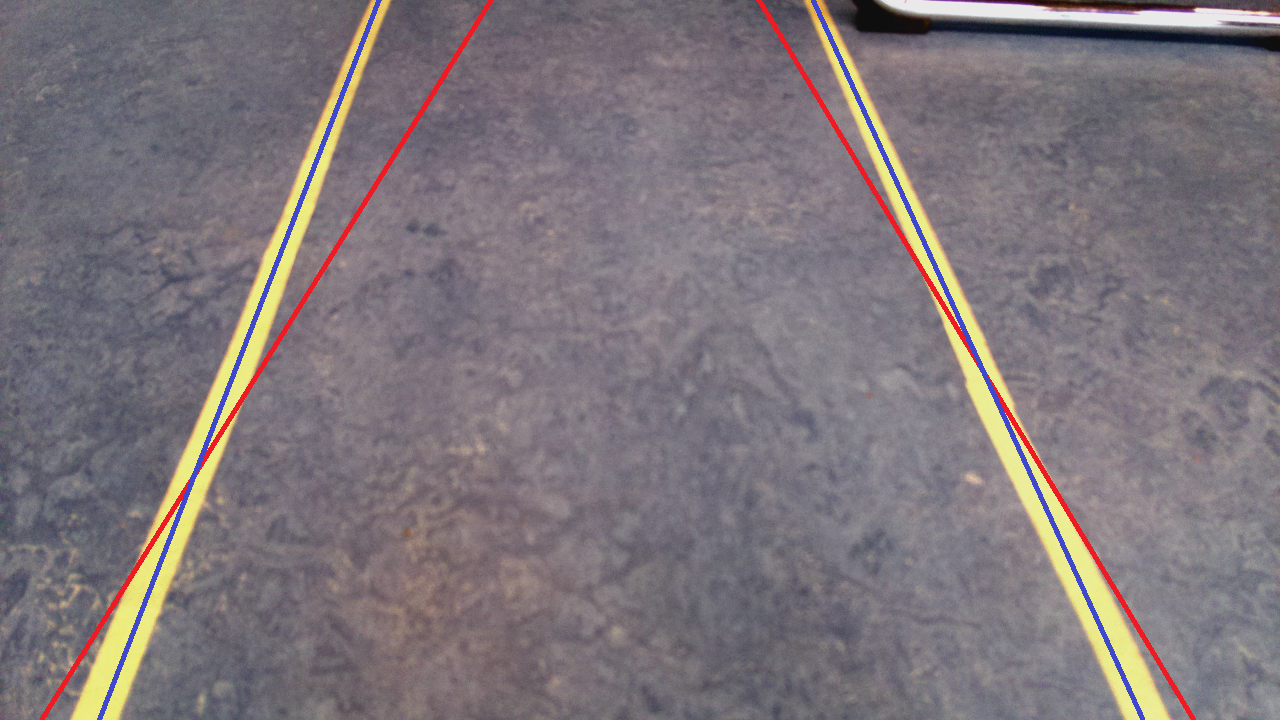
\includegraphics[width=.5\linewidth]{images/fahrbahn.png}
		\caption{Beispiel für die erste Form der Geradenrepräsentation}
		\label{fig:fahrbahn}
	\end{figure}
	
	
	Der Vergleich der Geraden wird durchgeführt, indem um die beiden Geraden aus dem letzten Durchlauf ein Toleranz-Fenster gelegt wird, und von allen gefundenen Geraden nur diejenigen herausgefiltert werden, die innerhalb dieses Toleranz-Fensters liegen. Von diesen Geraden wird dann der Durschnitt berechnet, sodass nur noch zwei Geraden für die beiden Fahrbahnlinien übrig bleiben. \\
	
	Eine Schwierigkeit besteht darin die Geraden so zu repräsentieren, dass diese gut miteinander vergleichbar sind. Bei einer geringen Änderung einer Geraden von einem zum nächsten Zyklus sollen sich deren Parameter dabei auch nur geringfügig ändern. Ansonsten werden ähnliche Geraden beim filtern verworfen, da deren Parameter nicht im Toleranzfenster liegen. Im Programm wurden daher je nach Anwendungsfall verschiedene Repräsentationsformen verwendet, welche im folgenden beschrieben werden.
	
	\subsection{Verwendete Repräsentationsformen von Geraden}
	
	Die Funktion HoughLines gibt als Ergebnis eine Liste von Geraden aus, die durch die beiden Parameter $\rho$ und $\theta$ beschrieben werden wird. $\theta$ ist der Winkel zwischen der Normalen, die senkrecht auf der Geraden steht, und der x-Achse. Der Winkel  $\rho$ ist die Länge dieser Normalen, d.h. der Abstand zwischen der Geraden und dem Ursprung des Koordinatensystems. Der Winkel $\theta$ ist immer positiv, $\rho$ kann, je nach Lage der Geraden positiv oder negativ sein.
	Abbildung \ref{fig:rho_theta1} zeigt ein Beispiel für die Repräsentation zweier Fahrbahnlinien in der $\rho$-$\theta$-Darstellung, für den Fall, dass der Wagen relativ mittig und gerade auf der Fahrbahn steht. Das Rechteck symbolisiert die Ränder des Kamerabildes. Der Koordinatenursprung liegt in der oberen linken Ecke. $\theta_R$ und $\rho_R$ sind die Parameter der rechten Fahrbahnlinie, $\theta_L$ und $\rho_L$ die der Linken.
	
	\begin{figure}[H]
		\centering
		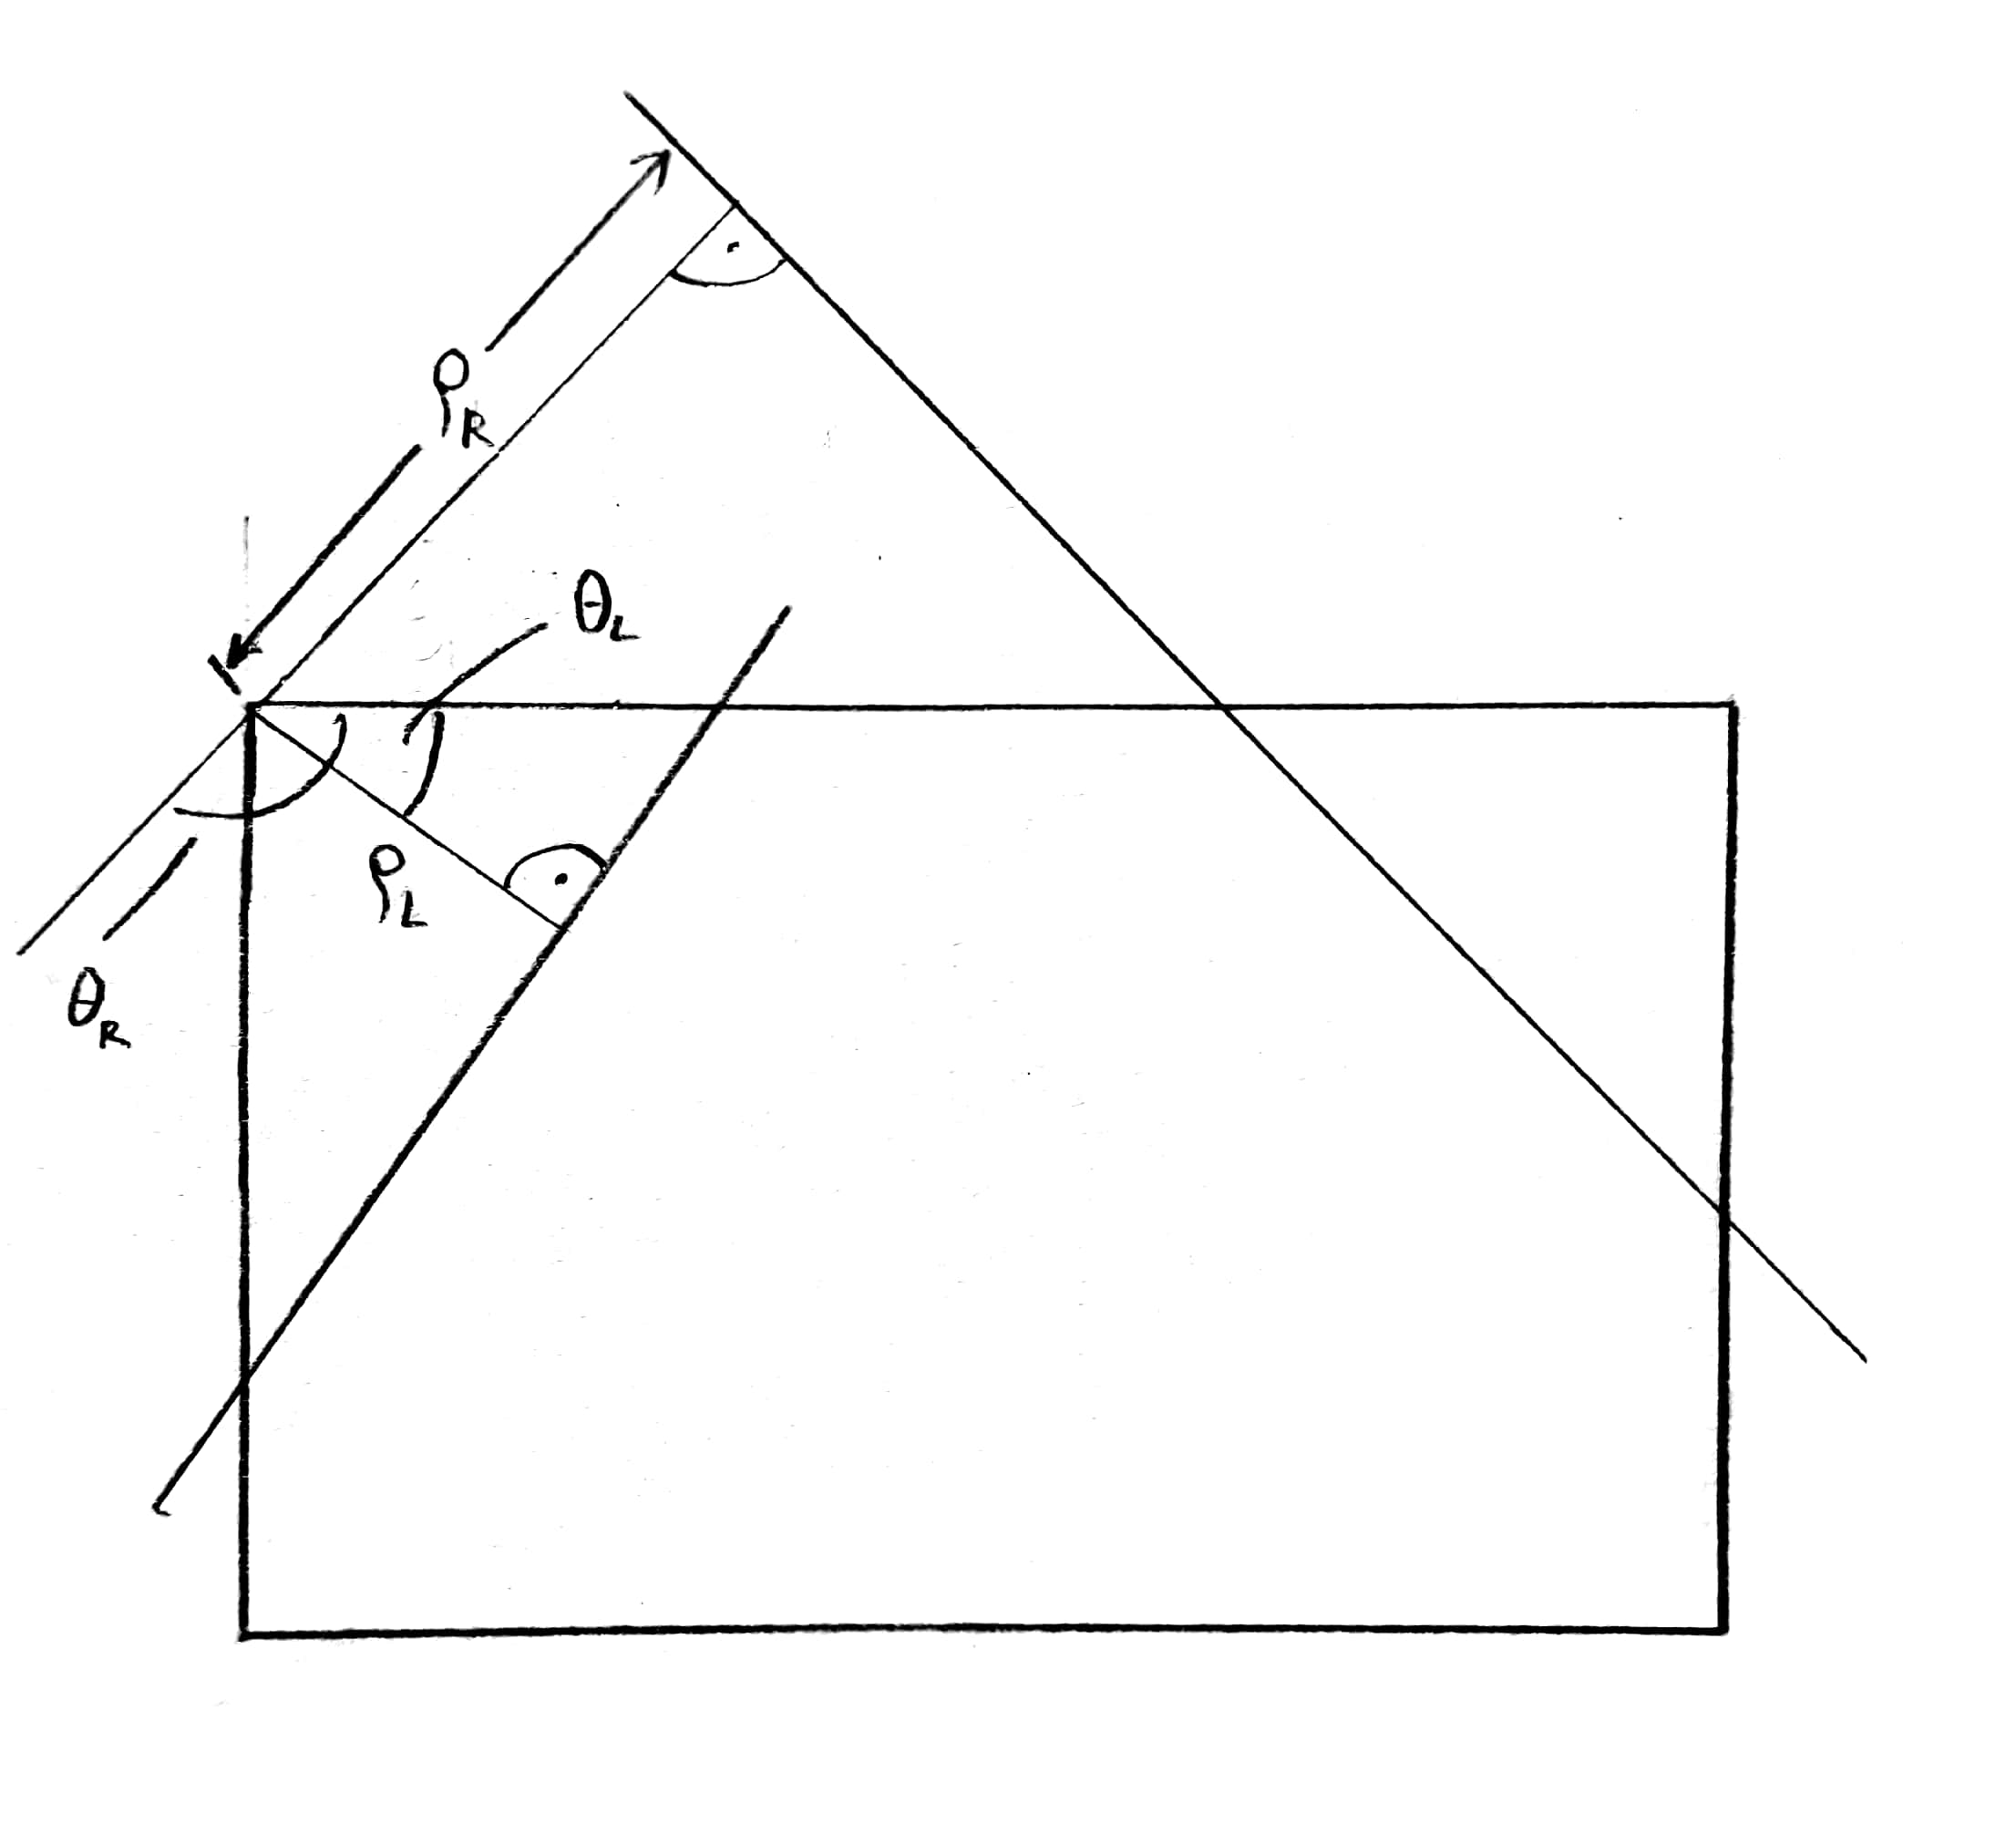
\includegraphics[width=.5\linewidth]{images/rho_theta1.jpg}
		\caption{Beispiel für die erste Form der Geradenrepräsentation}
		\label{fig:rho_theta1}
	\end{figure}
	
	Diese Form der Geradenrepräsentation jedoch problematisch, wenn es darum geht, zwei Geraden miteinander zu vergleichen. Ein Beispiel ist in Abbildung \ref{fig:rho_theta2} dargestellt. Hier beträgt die Änderung der Winkel $\theta_R$ und $\theta_L$ der beiden Fahrbahnlinien $\Delta\theta=5^\circ$, obwohl die Position der rechten Fahrbahnlinie sich viel mehr verändert hat, als die der linken.
	
	
	
	\begin{figure}[H]
		\centering
		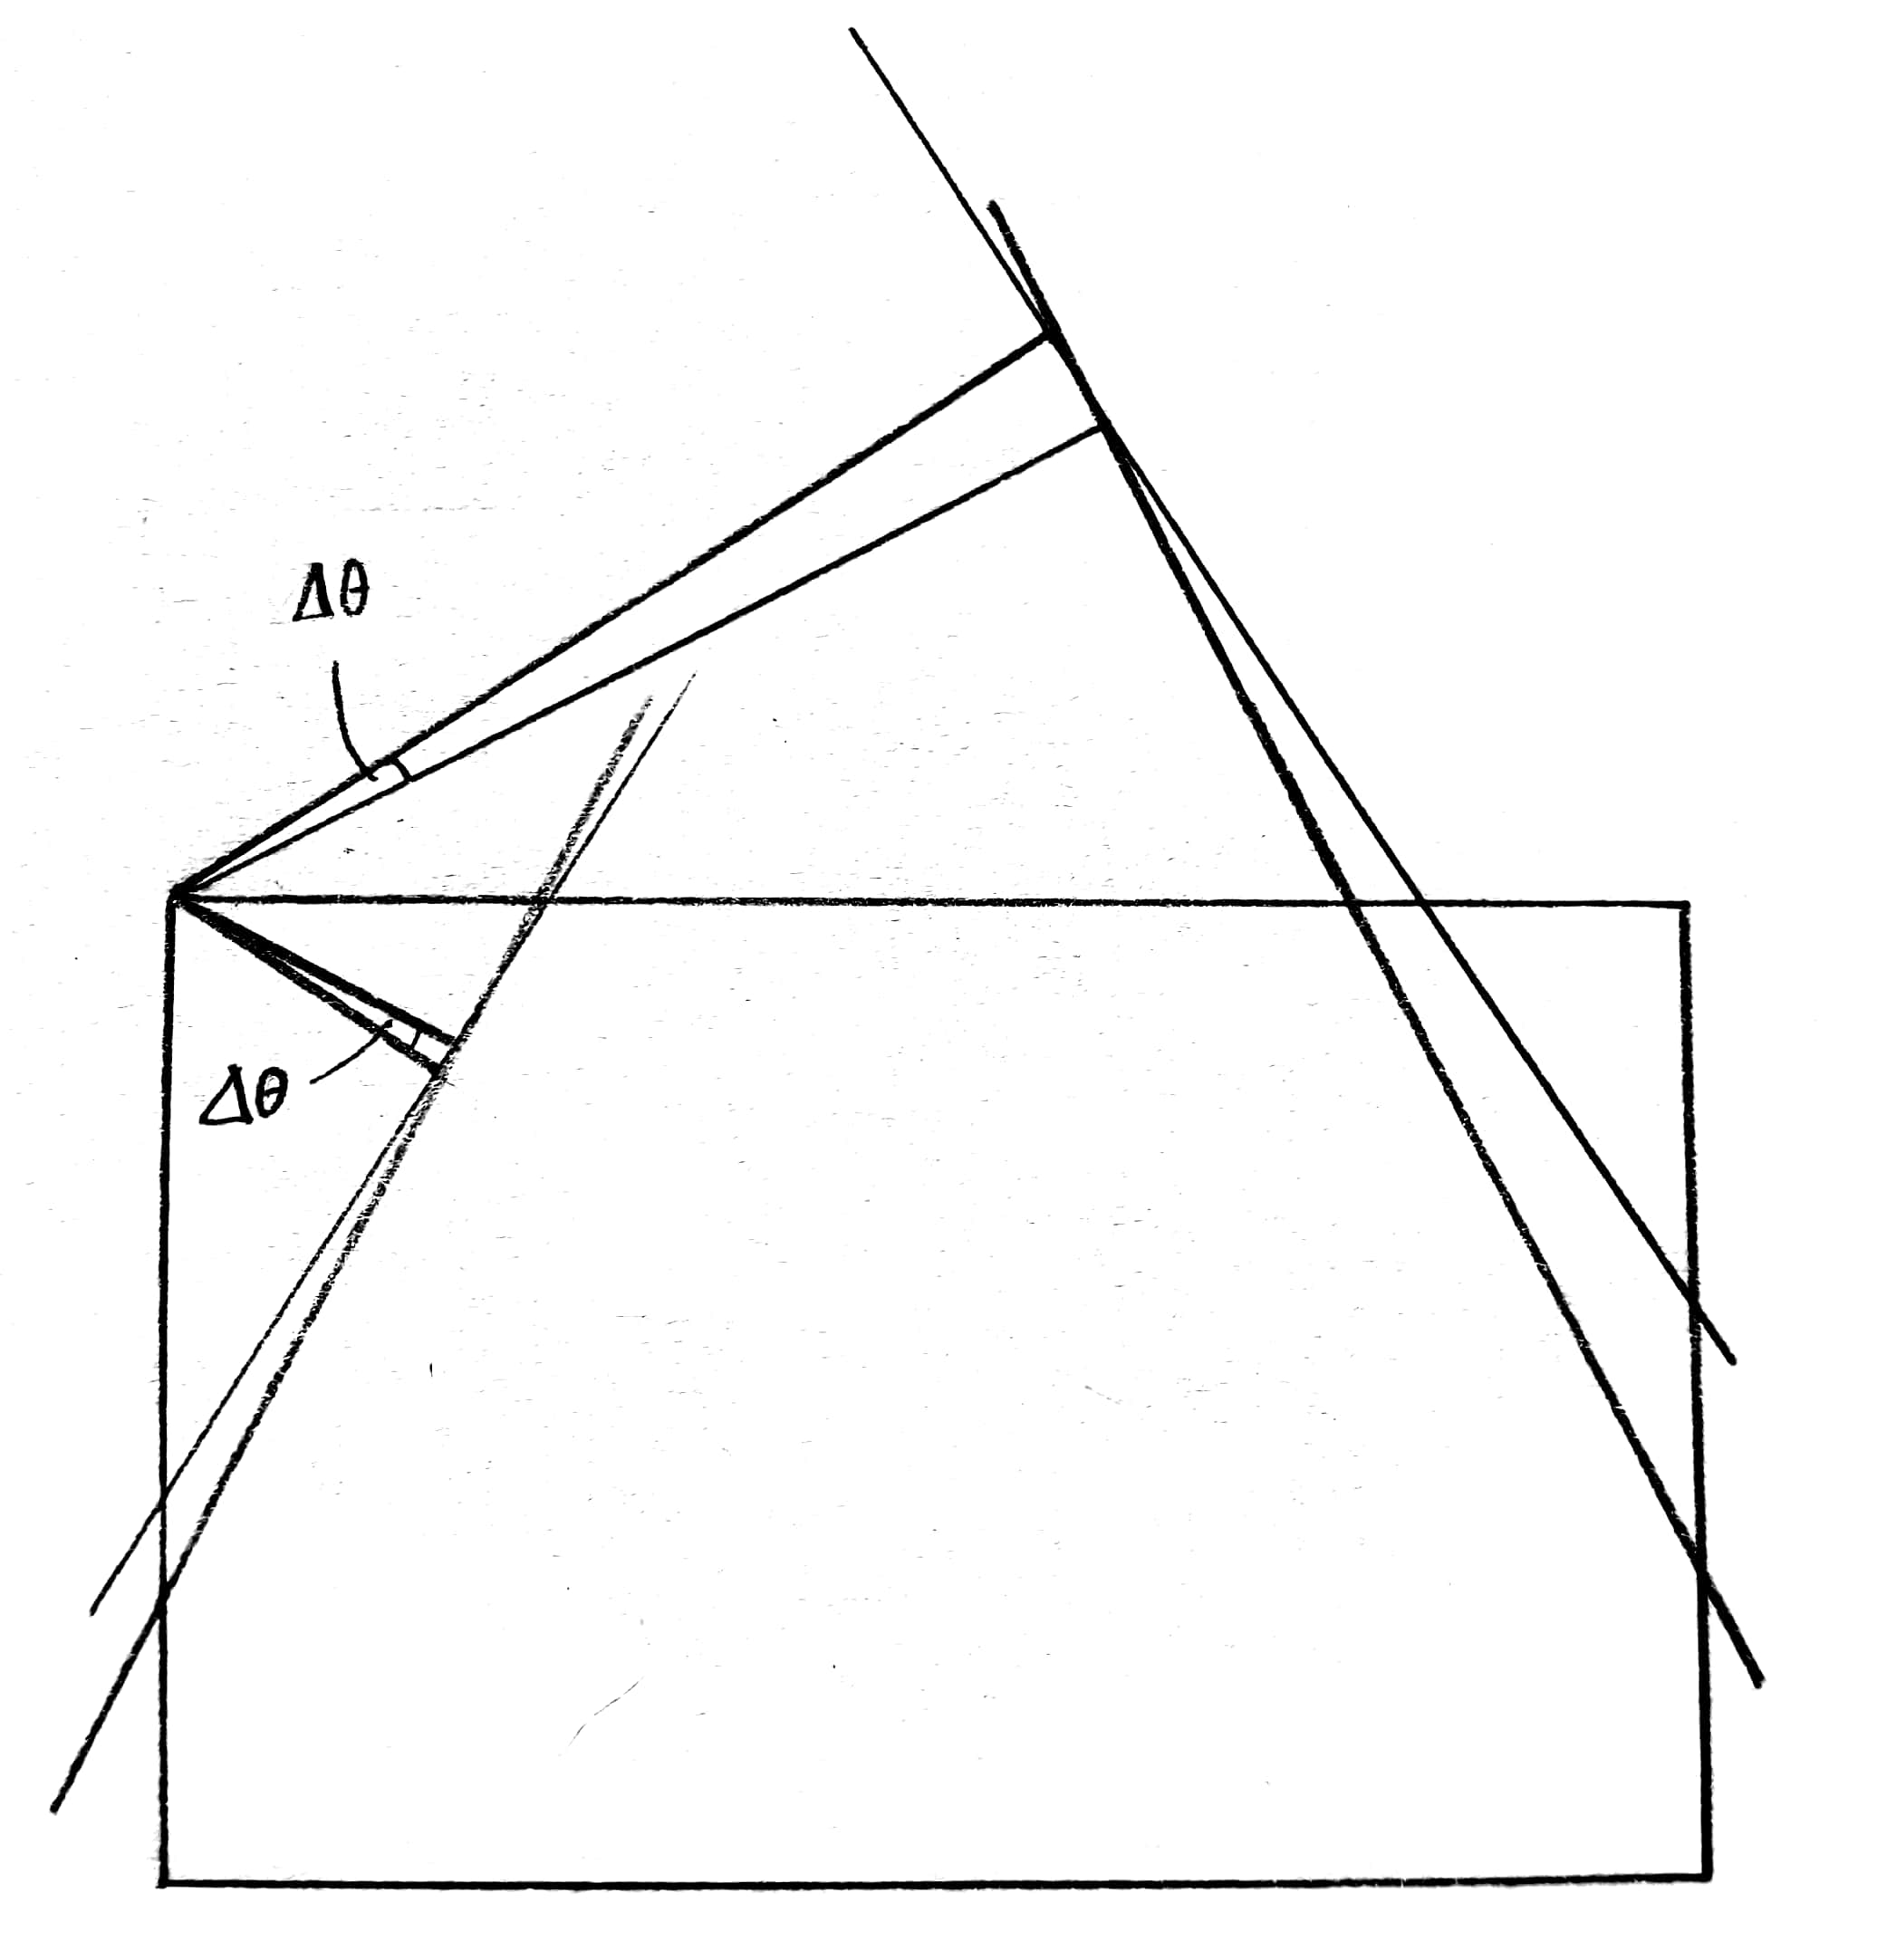
\includegraphics[width=.5\linewidth]{images/rho_theta2.jpg}
		\caption{Problematischer Fall für diese Form der Geradenrepräsentation}
		\label{fig:rho_theta2}
	\end{figure}

	Um dieses Problem zu beheben wurden die Geraden mithilfe der Funktion get\_offset\_alpha1 in eine andere Form umgerechnet, bei der diese durch den Offset $\omega$ auf der y-Achse und den Winkel zur x-Achse beschrieben werden. Die Umrechnung von der $\rho$-$\theta$-Form erfolgt folgendermaßen:\\

	
	
	Für Winkel $\theta<90^\circ$ (linke Fahrbahnlinie):
	
	\begin{align*}
	\alpha=90^{\circ}-\theta
	\omega&=-\frac{\rho}{\cos{90^{\circ}-\theta}} \\
	\end{align*}
	
	Für Winkel $\theta>90^\circ$ (rechte Fahrbahnlinie):
	
	\begin{align*}
	\alpha=\theta-90^{\circ}
	\omega&=-\frac{\rho}{\cos{\theta-90^{\circ}}} \\
	\end{align*}
	
	Abbildung \ref{fig:alpha_omega1} veranschaulicht die Repräsentation der beiden Fahrbahnlinien in dieser Form.
	
	\begin{figure}[H]
		\centering
		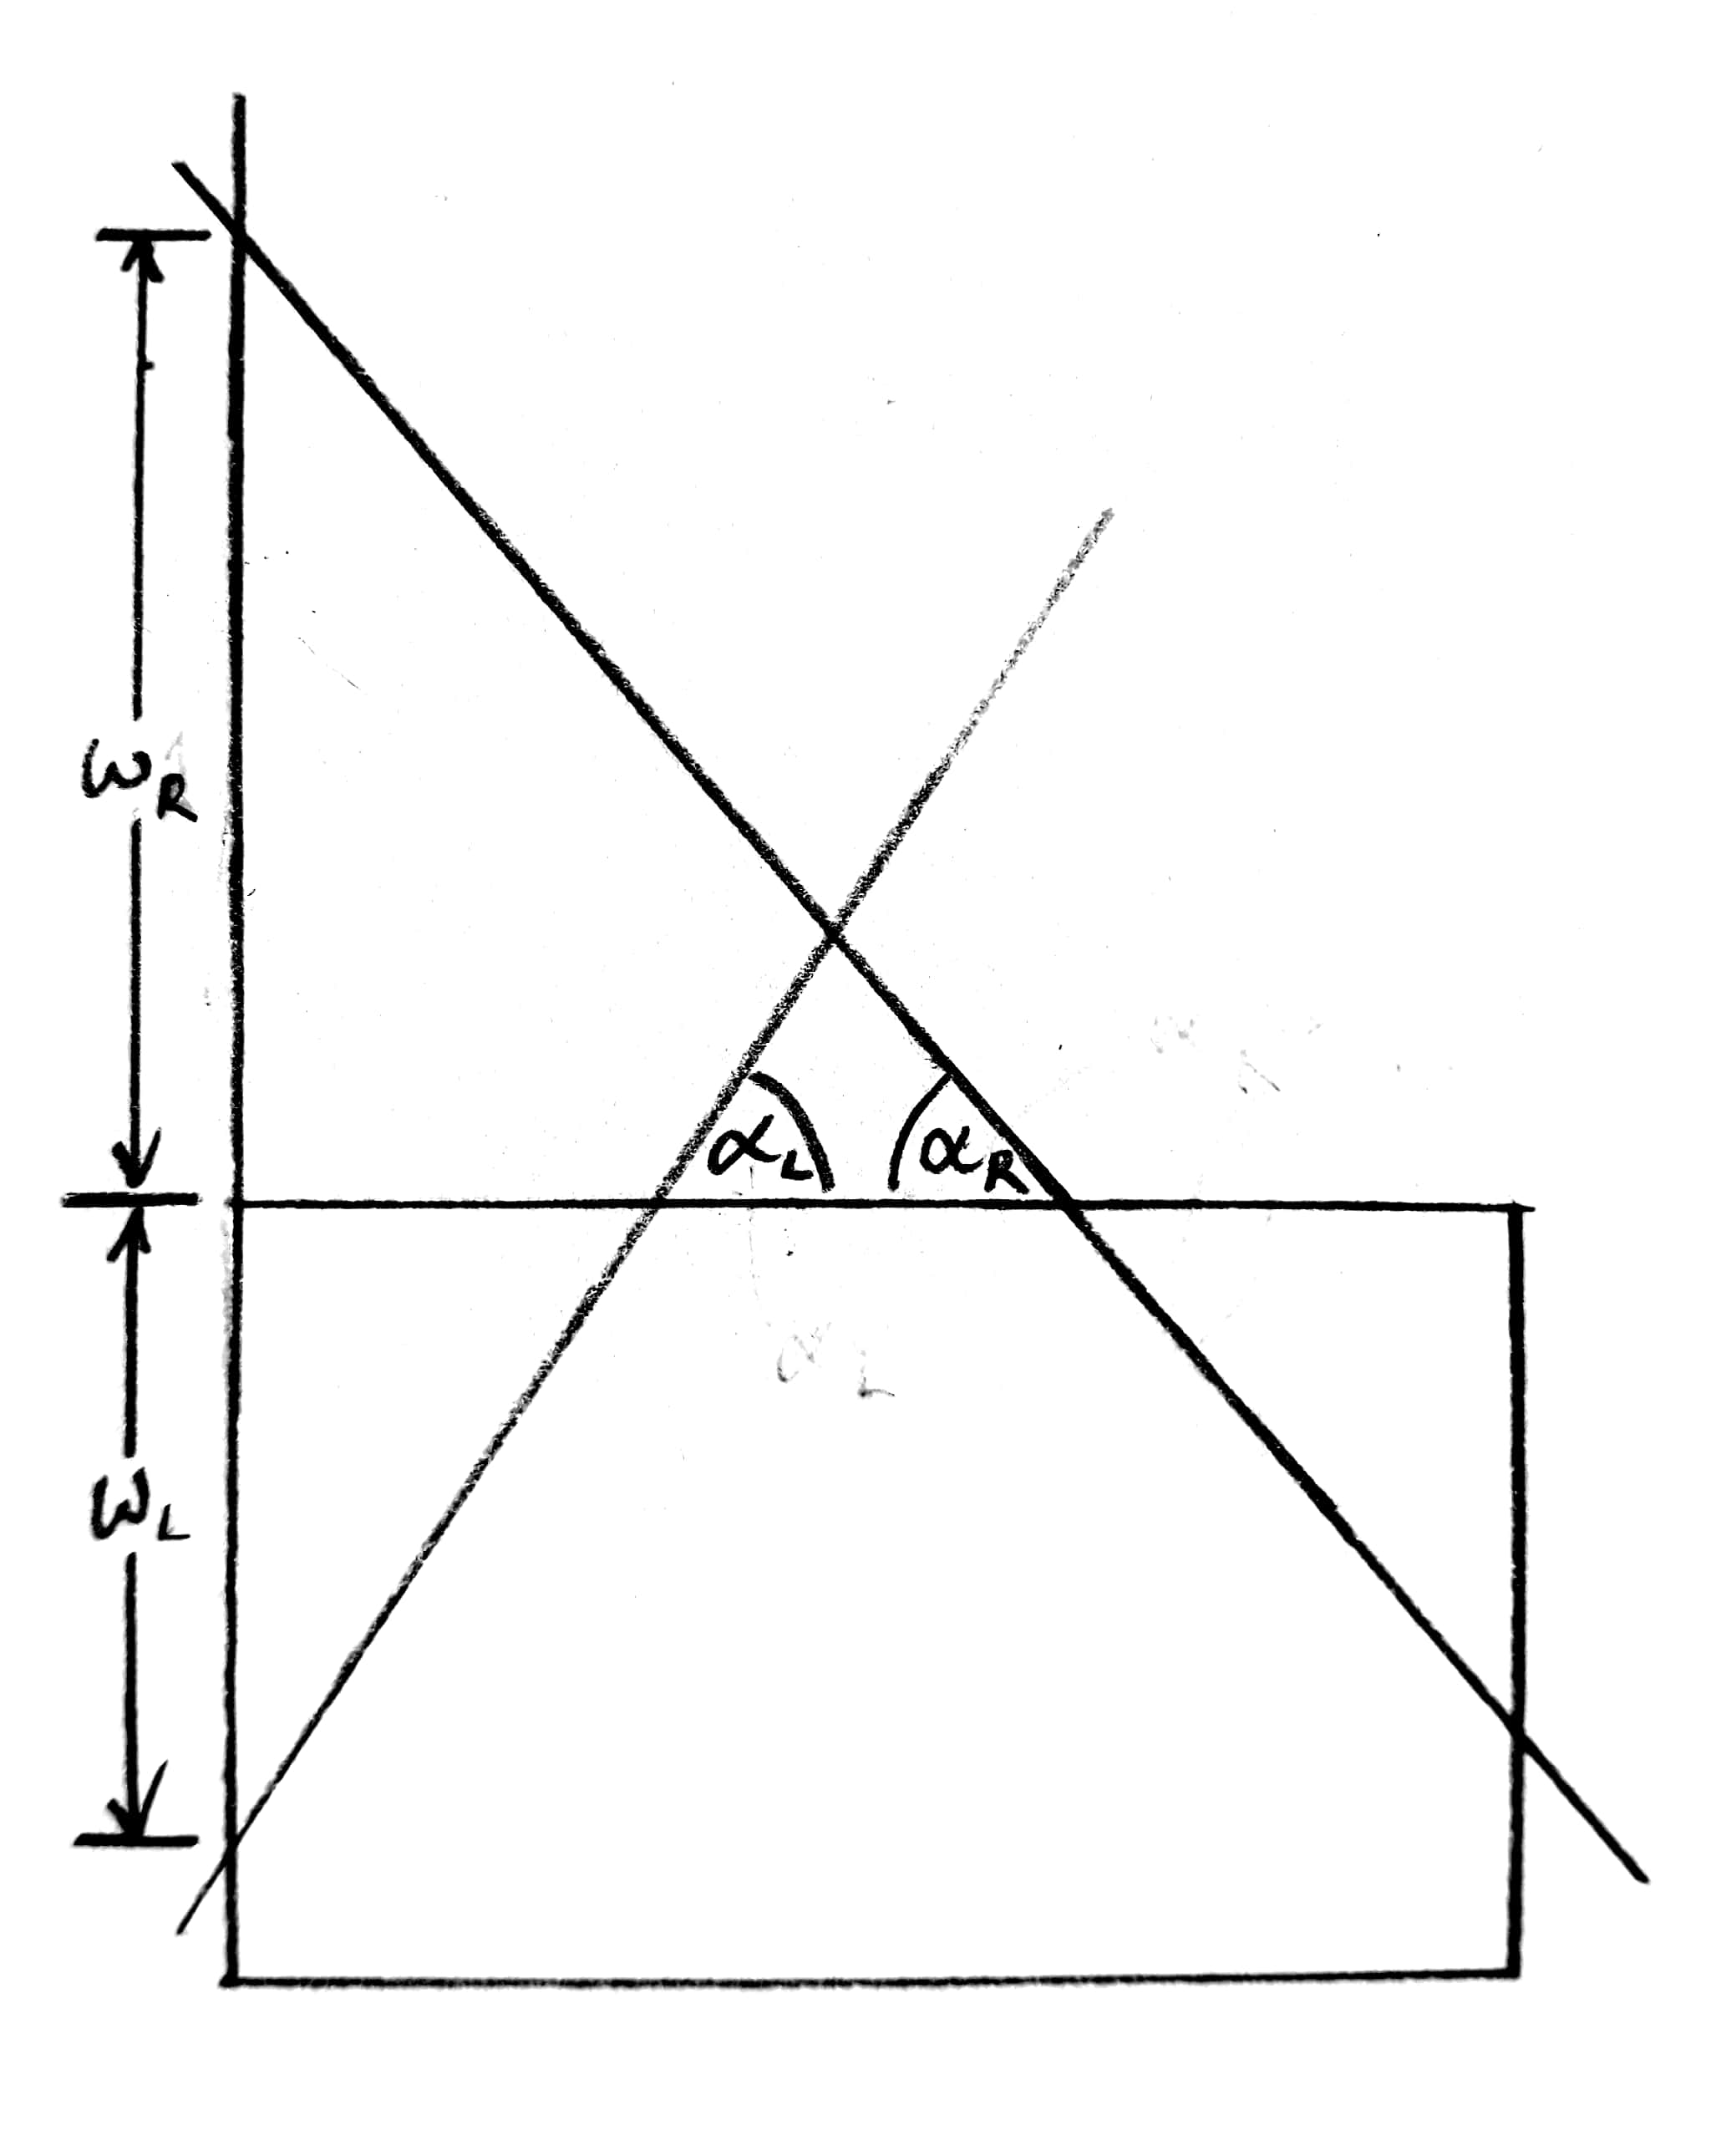
\includegraphics[width=.5\linewidth]{images/alpha_omega1.jpg}
		\caption{Beispiel für die erste Form der Geradenrepräsentation}
		\label{fig:alpha_omega1}
	\end{figure}

	Bei dieser Form ergibt sich jedoch das Problem, dass sich bei geringfügiger Veränderung der Geraden deren Parameter in bestimmten Situationen stark ändern. Dies ist besonders für die rechte Fahrbahnlinie der Fall, wie sich in Abbildung \ref{fig:alpha_omega2} erkennen lässt. Hier sieht man, dass sich der Offset $\omega$ stark ändert, auch wenn sich der Winkel der Geraden nur leicht ändert.


	\begin{figure}[H]
		\centering
		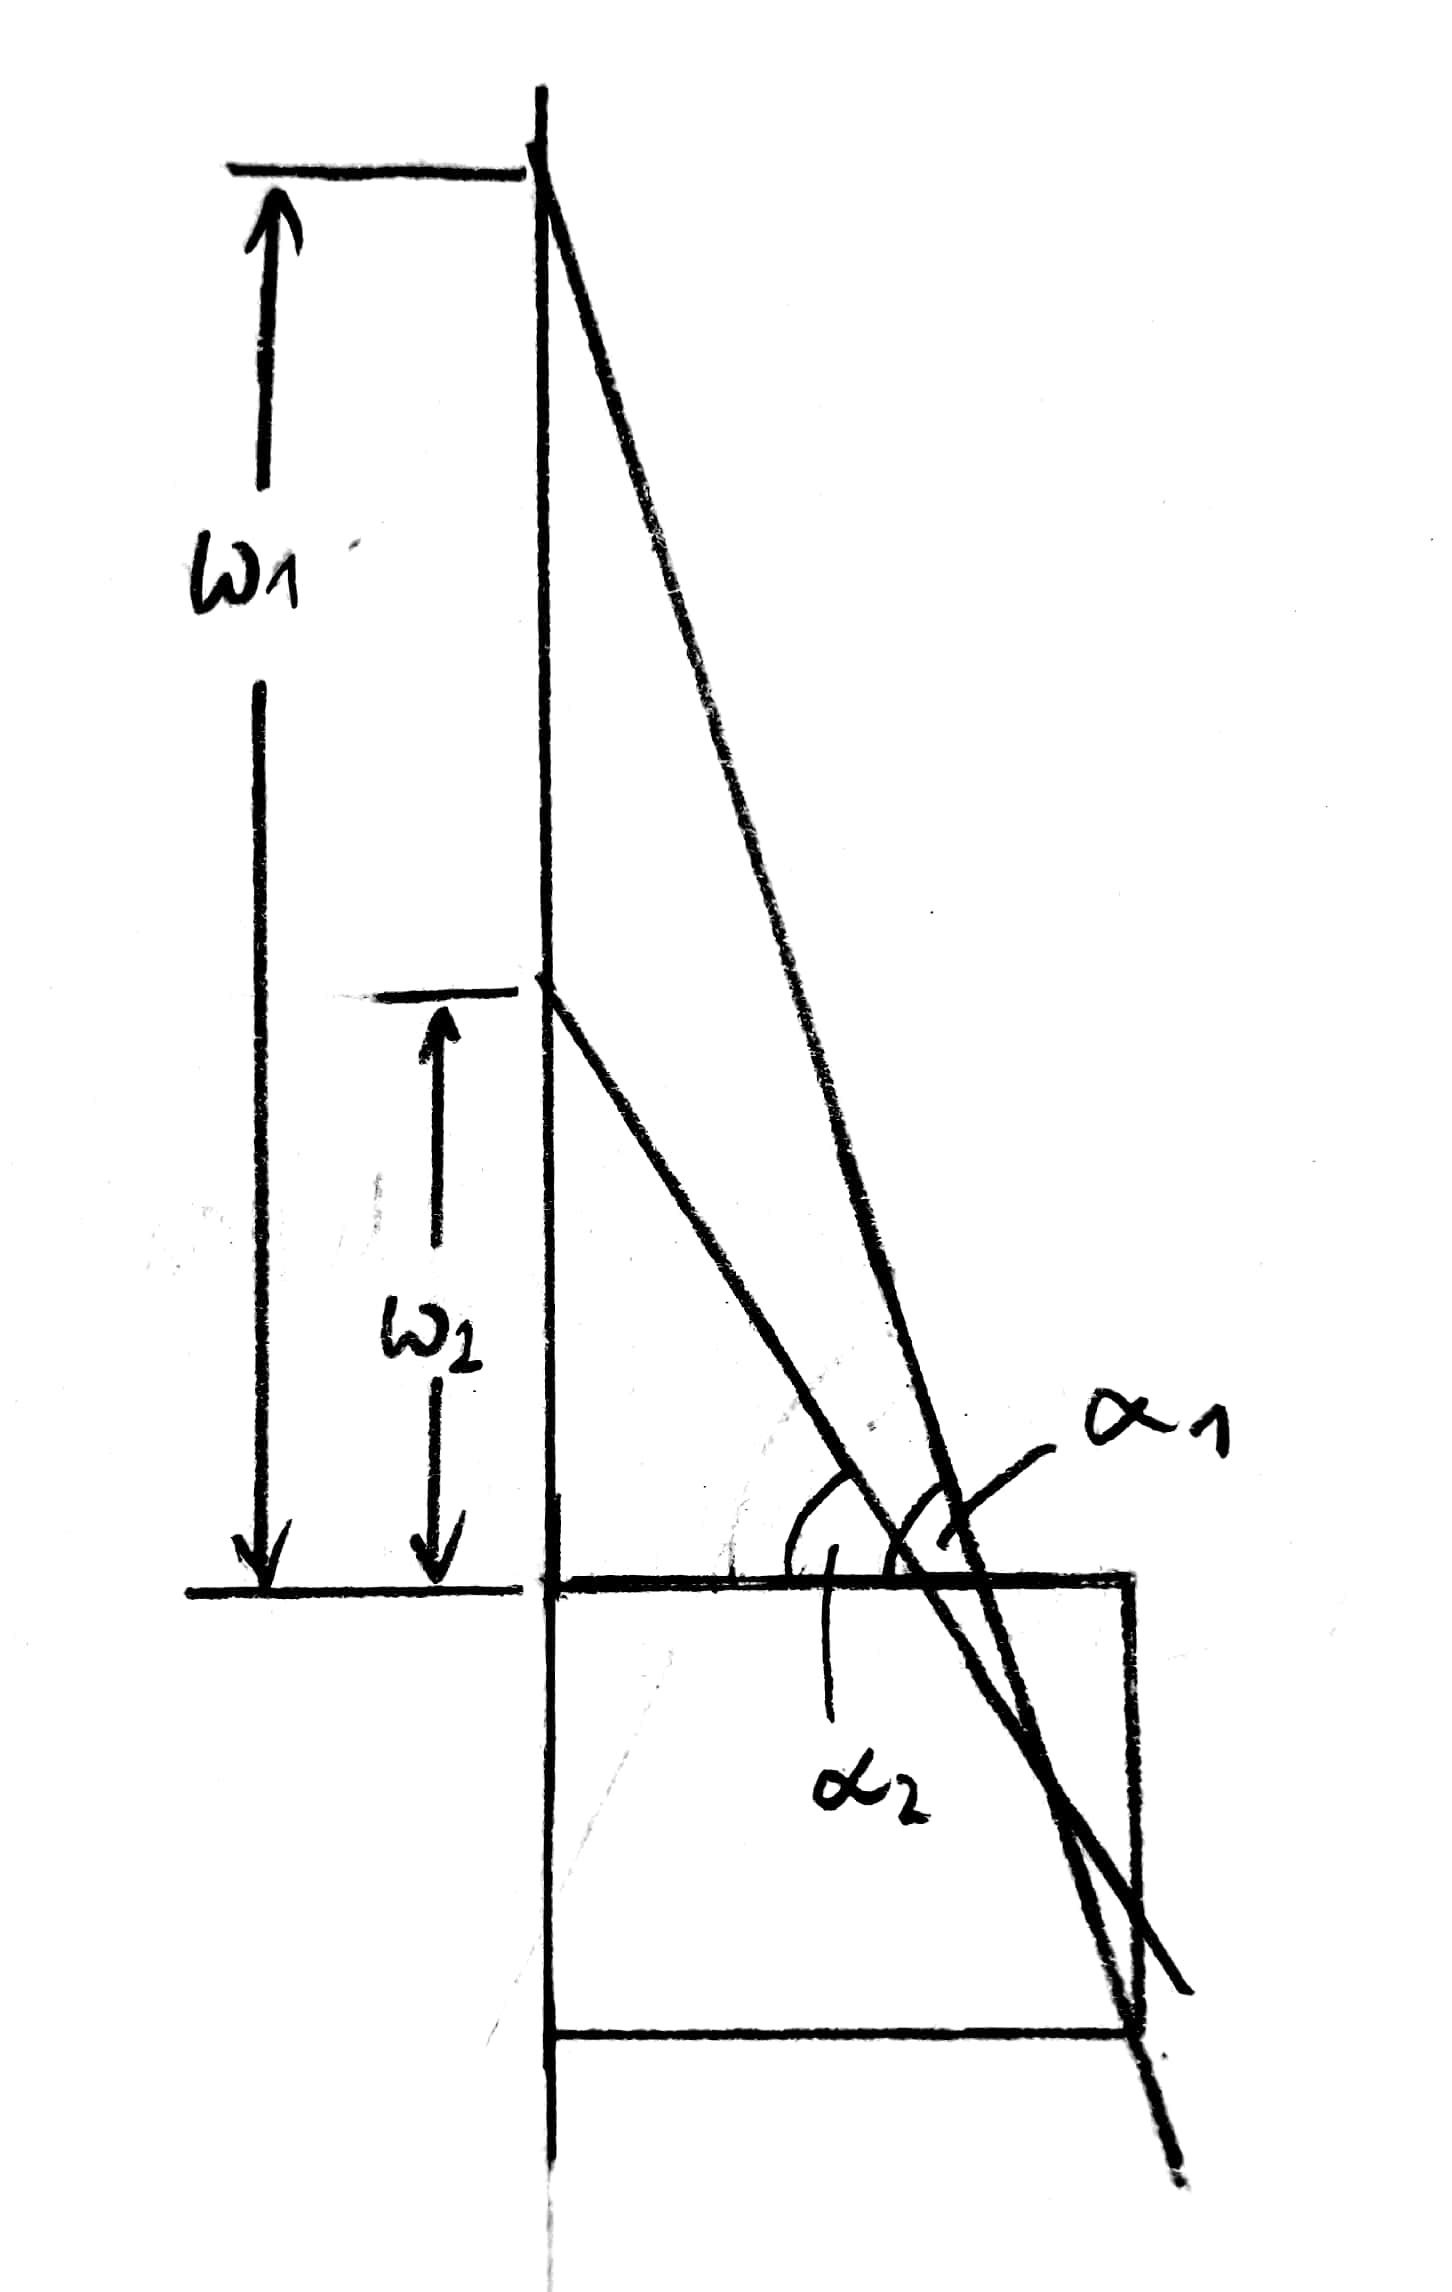
\includegraphics[width=.3\linewidth]{images/alpha_omega2.jpg}
		\caption{Beispiel für die erste Form der Geradenrepräsentation}
		\label{fig:alpha_omega2}
	\end{figure}

	Daher wurden für die beiden Geraden zwei verschiedene Repräsentationsformen gewählt. Für die Linke gerade wird der Offset von der linken oberen Ecke gemessen, für die rechte der Offset von der rechten oberen Ecke. Die Winkel werden wie gehabt zur x-Achse gemessen. In dieser Form lassen sich die Geraden am besten vergleichen. Die Umformung von der $\rho$-$\theta$-Form geschieht in der Funktion get\_offset\_alpha2 durch folgende Berechnungen: \\
	
	\begin{align*}
	\alpha=90^{\circ}-\theta
	\end{align*}
	
	
	Für Winkel $\theta<90^\circ$ (linke Fahrbahnlinie):
	
	\begin{align*}
	\omega&=-\frac{\rho}{\cos{90^{\circ}-\theta}} \\
	\end{align*}
	
	Für Winkel $\theta>90^\circ$ (rechte Fahrbahnlinie):
	
	\begin{align*}
	\omega&=\frac{B+\frac{\rho}{\cos{\theta-90^{\circ}}}}{\tan{90^{\circ}-\theta}} \\
	\end{align*}
	
	Mit der Bildbreite B.
	
	Abbildung \ref{fig:alpha_omega3} veranschaulicht diese Repräsentationsform.
	
		\begin{figure}[H]
		\centering
		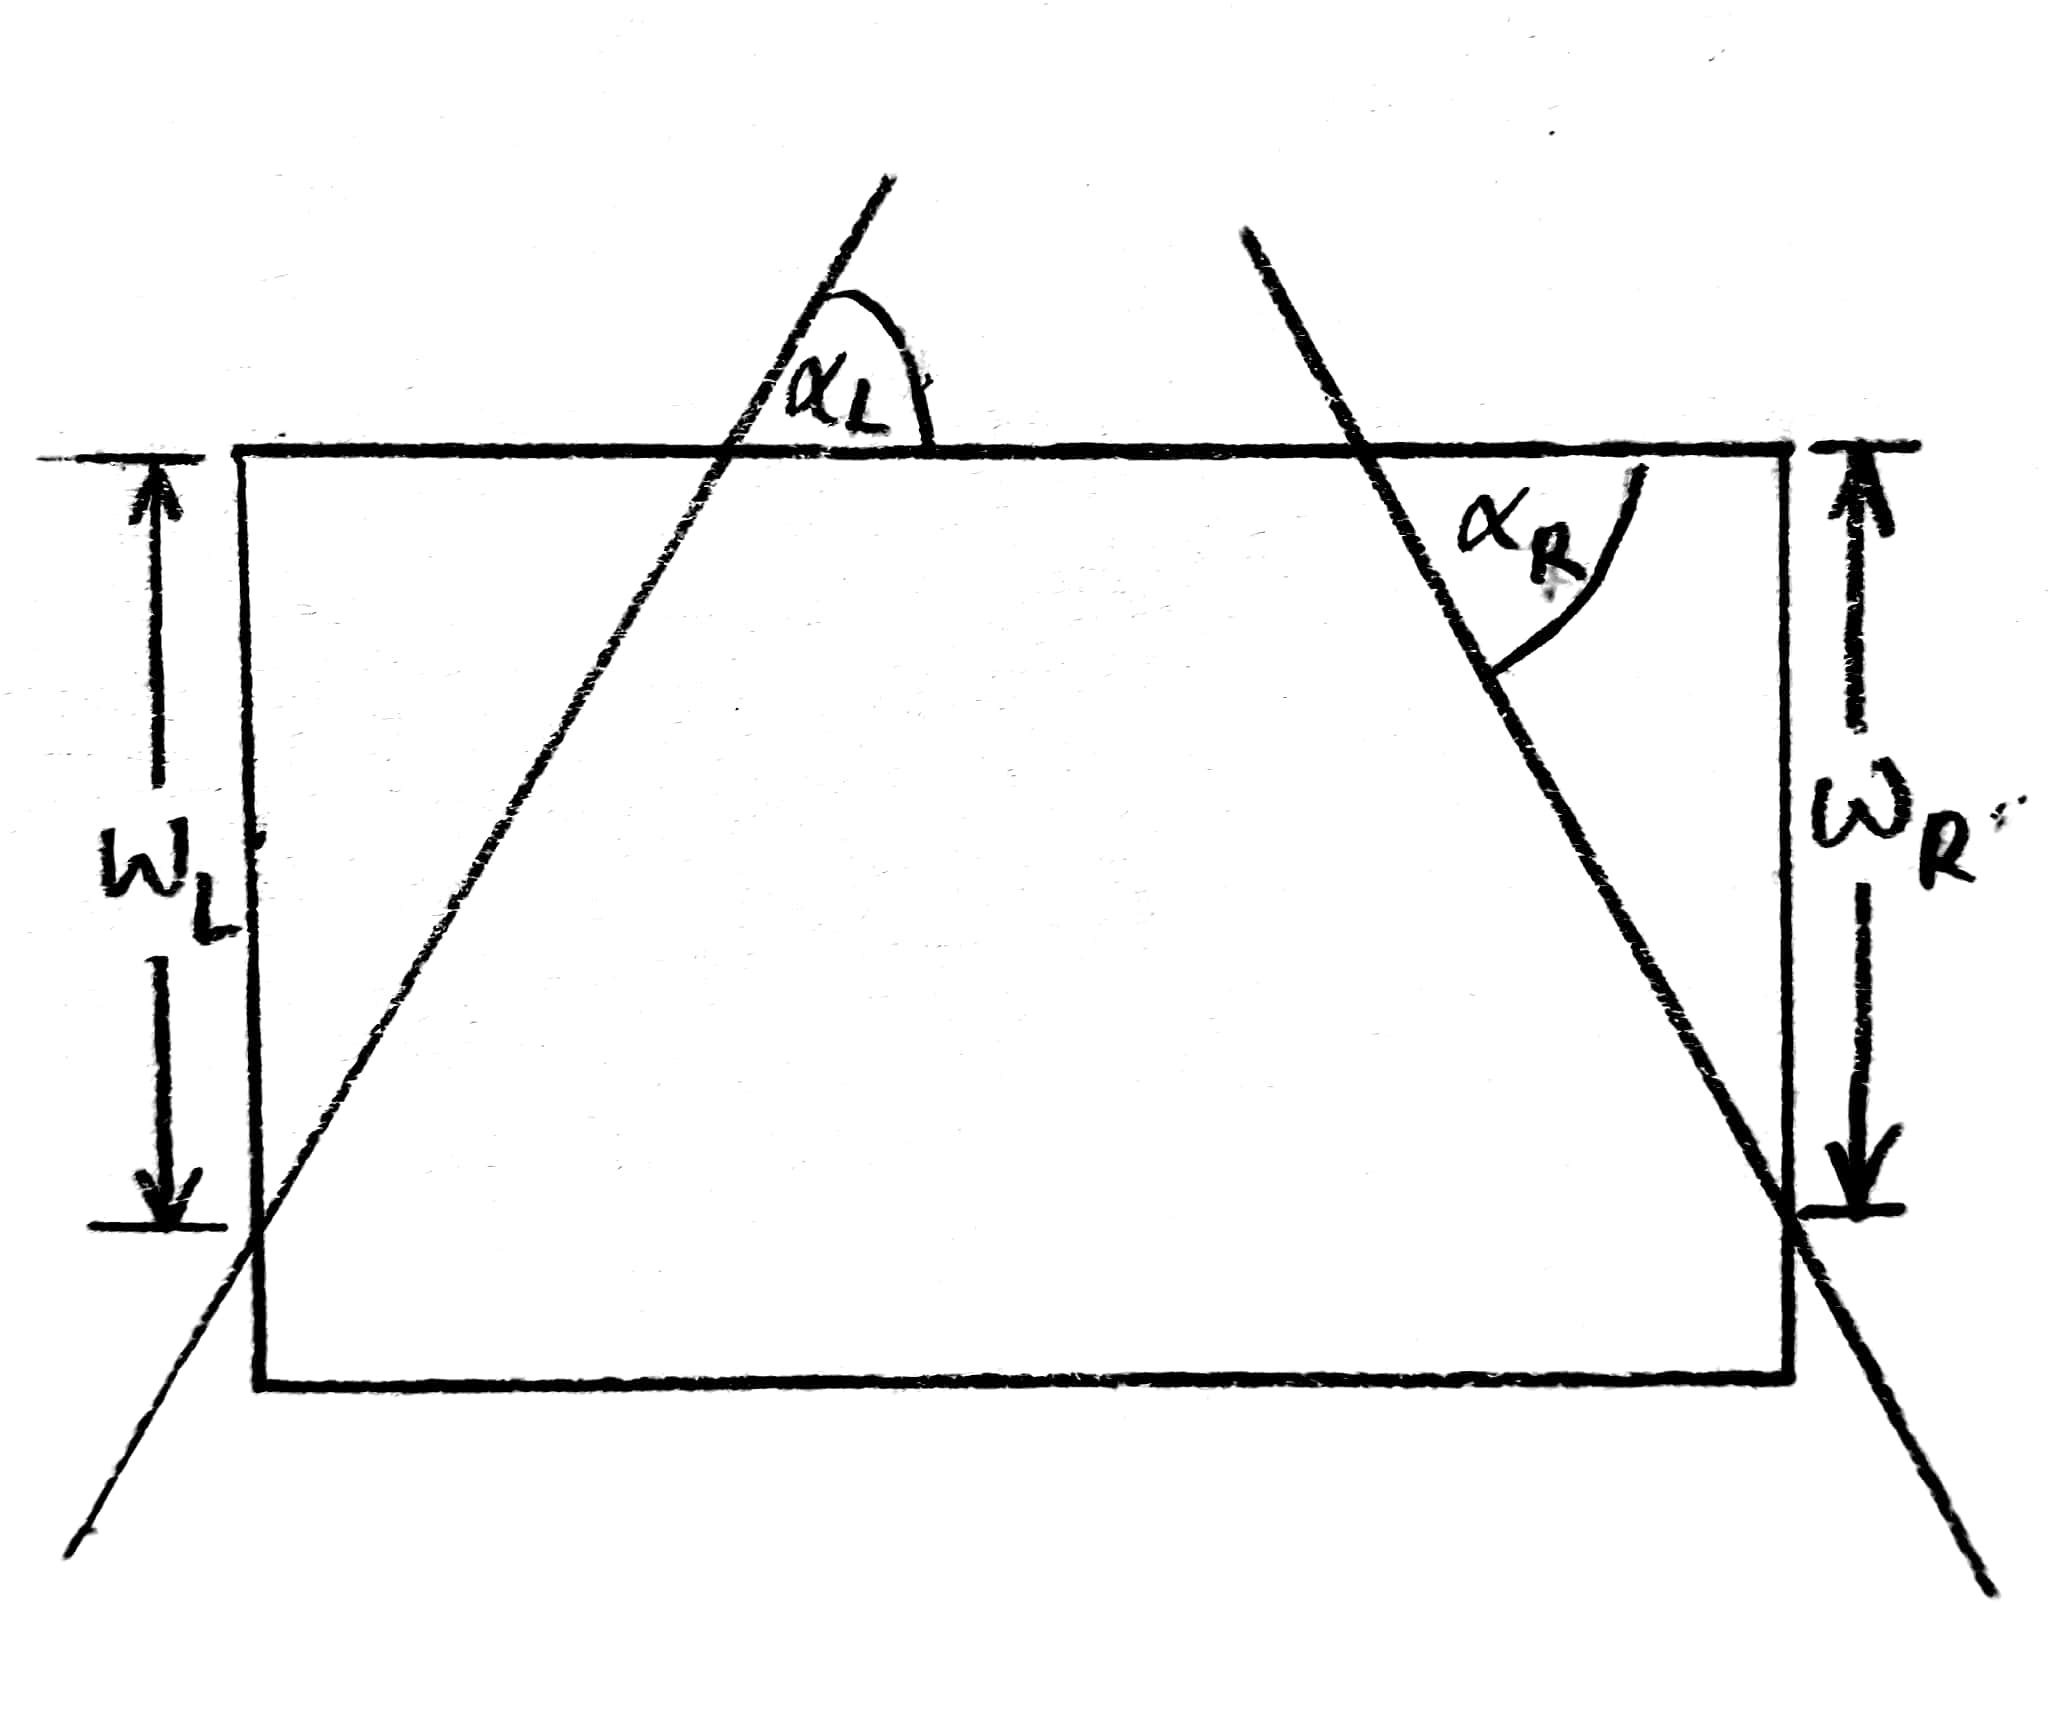
\includegraphics[width=.5\linewidth]{images/alpha_omega3.jpg}
		\caption{Beispiel für die erste Form der Geradenrepräsentation}
		\label{fig:alpha_omega3}
	\end{figure}


	\subsection{Berechnung des Schnittpunktes der beiden Geraden}
	
	Der Lenkwinkel wird mithilfe der x-Koordinate des Fluchtpunktes, also des Schnittpunktes der beiden Geraden berechnet. Die Abweichung dieses x-Wertes vom Mittelpunkt kann als Regeldifferenz verwendet werden.\\
	Die x-Koordinate des Fluchtpunktes (engl. vanishing point) wird in der Funktion get\_vp mit folgender Formel berechnet:\\
	
	\begin{align*}
	vp_x=\frac{\omega_R-\omega_L}{\tan{\alpha_L}+\tan{\alpha_R}} \\
	\end{align*}
	
	Um die Abweichung vom x-Wert der Bildmitte zu erhalten, wird von diesem Wert die Hälfte der Bildbreite B abgezogen:\\
	
	\begin{align*}
	Dx=vp_x-\frac{B}{2} \\
	\end{align*}
	
	
	
	
	
	
	
	
%	Beim Start des Programms werden für die beiden Geraden feste Werte vorgegeben. Anhand dieser Anfangswerte werden die im nächsten Durchlauf die Fahrbahnlinien durch bessere Werte angenähert.\\
%	Dafür wird das Bild zunächst mithilfe eines Schwellwertes in Schwarzweiß umgewandelt. Bei einem geeigneten Schwellwert sollten nun möglichst nur die beiden Fahrbahnlinien weiß sein (den Wert 1 haben).\\
%	Als nächstes wird die Funktion HoughLines aus der Bibliothek cv ausgeführt, die alle Geraden im Bild sucht. Die Funktion Houghlines gibt als Rückgabewert eine Liste von Geraden zurück, die in Polarkoordinaten durch einen Winkel $\rho$ und ein Abstand $\theta$ repräsentiert werden. $\rho$ ist der Winkel zwischen der Normalen, die senkrecht auf der Geraden steht, und der x-Achse. $\theta$ ist die Länge dieser Normalen, d.h. der Abstand zwischen der Geraden und dem Ursprung des Koordinatensystems.
	